In contrast to other methods, this methodology has been designed in such a way that the magnetic field \(\mathbf{B}\) needs to be calculated only once, but requires the inversion of a potentially large non-sparse matrix (performed using the backslash operator or \texttt{mldivide} function in MATLAB). As such, it is considerably faster than the iterative methods often seen in literature, but requires more computational memory. In addition, this method uses an analytical equation \cite{OConnell2020a} to calculate the magnetic field, making it faster than finite element methods to obtain an accurate solution.

\subsection{Computational speed}
To assess computation speed, a simple magnetic system was defined using two cube magnets in repulsion, separated by one magnet width, equivalent to Figure \ref{fig:p4cubeMagnetsRepulsion} with \(d = l\). To assess accuracy, the relative permeability of the magnets was set to unity, \(\mu_r = 1\), which allows the use of exact analytic force equations published by \textcite{Akoun1984}. The force was calculated using both the methodology defined in this paper, finite element simulations, and the exact force equations using MATLAB R2020a on a personal computer with an Intel Xeon E3-1240 v5 at 3.50GHz with 16GB of memory. The force calculations using finite element simulations and the methodology in this paper were repeated with varying mesh densities and timed to give an indication of computation speed. Both methods were compared to the exact analytic force equations \cite{Akoun1984} to give a measure of error, with both methods showing approximately the same rate of error convergence, but with the methodology in this paper giving results approximately an order of magnitude faster for the same accuracy. The percentage error between the estimated force using the method in this paper and exact force was computed and is displayed in Figure \ref{fig:p4calculationTime}.
\begin{figure}
	\centering
	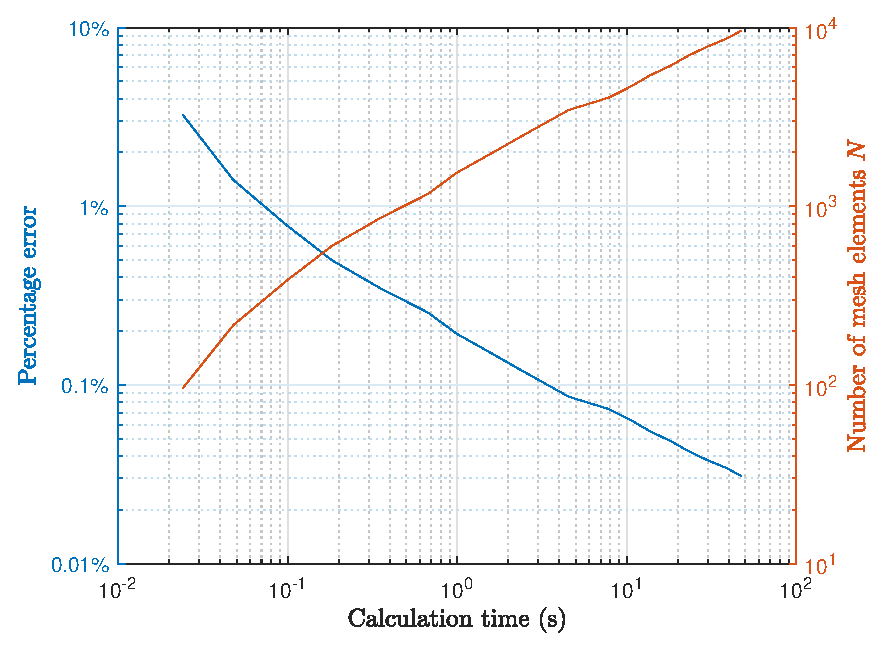
\includegraphics[width=0.8\linewidth]{p4/p4FIG13}
	\caption{Percentage error in the calculation of vertical force \(F_V\) between the magnets shown in Figure \ref{fig:p4cubeMagnetsRepulsion} with \(d = l\) and \(\mu_r = 1\) as mesh density, and thus calculation time, is increased. The number of surface mesh elements \(N\) is also plotted, showing an inverse trend when compared to the percentage error.}
	\label{fig:p4calculationTime}
\end{figure}

As expected, the percentage error decreases as calculation time increases. For this particular magnetic configuration and computation hardware, finite element simulations generally took more than 5s to achieve an error within 1\%. In contrast, the methodology in this paper took less than 100ms to attain less than 1\% error and less than 5s to attain less than 0.1\% error. This will vary depending on magnetic configuration, code implementation, and computation hardware, but gives an indication of the expected order of magnitude of calculation time to achieve a desired accuracy.

\subsection{Memory requirements}
This methodology requires more computational memory than other methods found in literature. Iterative methods, for example, require enough memory to keep track of the surface charge densities, but must recalculate the magnetic field information at each step. This can be done using a single \(N\times 1\) vector. In contrast, this method requires storing several large \(N\times N\) matrices of floating point numbers, as well as enough memory to invert a large \(\left(N+M\right) \times \left(N+M\right)\) matrix. This is a significantly larger memory requirement than iterative methods, but results in a considerably faster solution. During testing by the authors, a high precision calculation may use more than one gigabyte of memory, with equivalent finite element simulations requiring tens of gigabytes of memory. While considerable memory requirements are necessary for the method outlined in this paper, mesh optimisation was not considered. As such, testing was done using a basic mesh, with all elements being similar in size. If a more appropriate mesh is chosen, with finer mesh in areas with large magnetic field gradient, a high precision calculation can be done using less memory.

\subsection{Meshing considerations}
In this paper, a surface mesh has been used under the assumption that the magnetic permeability and remanence magnetisation vector are constant and uniform. If these assumptions are not valid, a volume mesh may be used and a similar methodology applied, where the magnetisation vector of each volume element is computed rather than the scalar surface charge density. However, the use of a volume mesh rather than surface mesh comes with a more considerable computation cost. Solving for the magnetisation vector field requires solving a large linear equation for each of the three Cartesian directions, while the scalar surface charge density solution only requires a single linear equation. In addition, calculation of the field produced by each element would require either using an inaccurate point dipole model, or calculating the field contribution from each of the surfaces of the element \cite{OConnell2020,OConnell2020a}. The use of the point dipole model considerably decreases accuracy for nearby elements, and the more complicated method considerably increases calculation time. These factors lead to a significantly larger computation cost when applying a volume mesh and solving the magnetisation vector field. Thus, for systems with constant and uniform permeability and remanence magnetisation, a surface charge density approach is preferred.

The methodology in this work uses a triangular surface mesh generated by finding the minimum convex hull of a set of vertices using the Geom3D library in the MatGeom package in MATLAB \cite{Legland2021}. Subdivision of the surface mesh is performed by dividing each triangular element into four congruent triangles until a desired number of surface elements was achieved. A triangular surface mesh has been chosen since analytic field equations are available for these elements \cite{OConnell2020a,OConnell2020}. These equations may be used to solve for the field produced by a triangle with constant surface charge density, and are highly efficient, especially when many field calculations are performed. In addition, a triangular surface mesh can represent any polyhedral surface and can be used to approximate curved surfaces, enabling the approximate solution of any magnetic configuration. The meshing algorithm itself is out of the scope of this work, since it is focused only on calculating the charge densities on each surface element and the resulting fields, forces, and torques. However, alternative meshing algorithms may be applied, and future analysis could be done on optimising the meshing process for this methodology.
